\section{Esperimenti}

\subsection{Dataset utilizzati}
\subsubsection{LFM1b}


LFM1b\_artist è un dataset contenente informazioni riguardanti le interazioni tra utenti e artisti musicali.

\noindent Descrizione del dataset
\begin{table}[H]
    \centering
    \footnotesize
    \begin{tabularx}{\textwidth}{|c|X|}
        \hline
        \textbf{Feature} & \textbf{Descrizione} \\
        \hline
        n\_users & 120322 \\
        \hline
        n\_items & 3123496 \\
        \hline
        n\_inter & 65133026 \\
        \hline
        sparsity & 0.9998266933373666 \\
        \hline
        avg\_inter\_user & 541.3226675088513 \\
        \hline
    \end{tabularx}
    \caption{Informazioni sul dataset LFM1b\_artist}
    \label{tab:dataset_info}
\end{table}


\noindent Descrizione del knowledge graph
\begin{table}[H]
    \centering
    \footnotesize
    \begin{tabularx}{\textwidth}{|c|X|}
        \hline
        n\_ent\_head & 823213 \\
        \hline
        n\_ent\_tail & 353607 \\
        \hline
        n\_rel & 8 \\
        \hline
        n\_triple & 2114049 \\
        \hline
    \end{tabularx}
    \caption{Informazioni sul knowledge graph del dataset LFM1b\_artist}
    \label{tab:dataset_info}
\end{table}



\paragraph{Descrizione procedimento di pre-processing}


\noindent Il dataset originale risultava essere troppo grande per le risorse a nostra disposizione, dunque è stato opportunamente processato. In paritcolare sono state svolte le seguenti operazioni
\begin{itemize}
    \item \textbf{Filtraggio:} il dataset è stato filtrato eliminando tutte le interazioni in cui erano coinvolti utenti e/o item con meno di 5 interazioni
    \item \textbf{Sampling:} dopo la fase di filtraggio, è stato effettuato un sampling casuale il cui scopo era quello di ridurre il numero di utenti e di item presenti. In particolare sono stati selezionati casualmente 20000 utenti e 50000 item e sono state mantenute solo le interazioni in cui erano coinvolti utenti e item selezionati
\end{itemize}

\noindent In questo modo è stato ottenuto un dataset più piccolo e più facilmente gestibile rispetto a quello originale.
Per poter lavorare su più dataset si è deciso di effettuare un ulteriore processing del dataset, andando a creare dei sampling con una strategia di stratificazione: \footnote{{{Mantenendo il numero di utenti inalterato per ognuno di essi sono stati campionati casualmente un determinato numero di interazioni cercando di mantenere inalterati i "rapporti originali" tra i diversi utenti}}}{}
\begin{itemize}
    \item \textbf{75\%:} Per ogni utente sono state mantenute il 75\% delle interazioni originali
    \item \textbf{50\%:} Dal dataset al 75\% sono state mantenute circa il 66.67\% delle interazioni di ogni utente, in modo tale da avere il 50\% delle interazioni originali
    \item \textbf{25\%:} Dal dataset al 50\% sono state mantenute il 50\% delle interazioni di ogni utente, in modo tale da avere il 25\% delle interazioni originali
\end{itemize}


\noindent\textbf{Dataset 20.000 users, 50.000 items}

\noindent Descrizione del dataset
\begin{table}[H]
    \centering
    \footnotesize
    \begin{tabularx}{\textwidth}{|c|X|}
        \hline
        \textbf{Feature} & \textbf{Descrizione} \\
        \hline
        n\_users & 19841 \\
        \hline
        n\_items & 42457 \\
        \hline
        n\_inter & 900212 \\
        \hline
        sparsity & 0.9989313587429705 \\
        \hline
        avg\_inter\_user & 45.371301849705155 \\
        \hline
    \end{tabularx}
    \caption{Informazioni sul dataset LFM1b\_artist\_20U50I}
    \label{tab:dataset_info}
\end{table}


\noindent Descrizione del knowledge graph
\begin{table}[H]
    \centering
    \footnotesize
    \begin{tabularx}{\textwidth}{|c|X|}
        \hline
        n\_ent\_head & 15509 \\
        \hline
        n\_ent\_tail & 35156 \\
        \hline
        n\_rel & 5 \\
        \hline
        n\_triple & 46827 \\
        \hline
    \end{tabularx}
    \caption{Informazioni sul knowledge graph del dataset LFM1b\_artist\_20U50I}
    \label{tab:dataset_info}
\end{table}

\noindent\textbf{Dataset 75\%}

\noindent Descrizione del dataset
\begin{table}[H]
    \centering
    \footnotesize
    \begin{tabularx}{\textwidth}{|c|X|}
        \hline
        \textbf{Feature} & \textbf{Descrizione} \\
        \hline
        n\_users & 19841 \\
        \hline
        n\_items & 38932 \\
        \hline
        n\_inter & 667850 \\
        \hline
        sparsity & 0.9991354130849345 \\
        \hline
        avg\_inter\_user & 33.660097777329774 \\
        \hline
    \end{tabularx}
    \caption{Informazioni sul dataset LFM1b\_artist\_20U50I\_75strat}
    \label{tab:dataset_info}
\end{table}


\noindent Descrizione del knowledge graph
\begin{table}[H]
    \centering
    \footnotesize
    \begin{tabularx}{\textwidth}{|c|X|}
        \hline
        n\_ent\_head & 14327 \\
        \hline
        n\_ent\_tail & 32981 \\
        \hline
        n\_rel & 5 \\
        \hline
        n\_triple & 43559 \\
        \hline
    \end{tabularx}
    \caption{Informazioni sul knowledge graph del dataset LFM1b\_artist\_20U50I\_75strat}
    \label{tab:dataset_info}
\end{table}

\noindent\textbf{Dataset 50\%}

\noindent Descrizione del dataset
\begin{table}[H]
    \centering
    \footnotesize
    \begin{tabularx}{\textwidth}{|c|X|}
        \hline
        \textbf{Feature} & \textbf{Descrizione} \\
        \hline
        n\_users & 19841 \\
        \hline
        n\_items & 33653 \\
        \hline
        n\_inter & 440620 \\
        \hline
        sparsity &  0.9993401019218887 \\
        \hline
        avg\_inter\_user & 22.20755002268031 \\
        \hline
    \end{tabularx}
    \caption{Informazioni sul dataset LFM1b\_artist\_20U50I\_50strat}
    \label{tab:dataset_info}
\end{table}


\noindent Descrizione del knowledge graph
\begin{table}[H]
    \centering
    \footnotesize
    \begin{tabularx}{\textwidth}{|c|X|}
        \hline
        n\_ent\_head & 12522 \\
        \hline
        n\_ent\_tail & 29509 \\
        \hline
        n\_rel & 5 \\
        \hline
        n\_triple & 38491 \\
        \hline
    \end{tabularx}
    \caption{Informazioni sul knowledge graph del dataset LFM1b\_artist\_20U50I\_50strat}
    \label{tab:dataset_info}
\end{table}

\noindent\textbf{Dataset 25\%}

\noindent Descrizione del dataset
\begin{table}[H]
    \centering
    \footnotesize
    \begin{tabularx}{\textwidth}{|c|X|}
        \hline
        \textbf{Feature} & \textbf{Descrizione} \\
        \hline
        n\_users & 19841 \\
        \hline
        n\_items & 24878 \\
        \hline
        n\_inter & 218457 \\
        \hline
        sparsity & 0.9995574249320202 \\
        \hline
        avg\_inter\_user & 11.01038254120256 \\
        \hline
    \end{tabularx}
    \caption{Informazioni sul dataset LFM1b\_artist\_20U50I\_25strat}
    \label{tab:dataset_info}
\end{table}


\noindent Descrizione del knowledge graph
\begin{table}[H]
    \centering
    \footnotesize
    \begin{tabularx}{\textwidth}{|c|X|}
        \hline
        n\_ent\_head & 9444 \\
        \hline
        n\_ent\_tail & 23463 \\
        \hline
        n\_rel & 5 \\
        \hline
        n\_triple & 29822 \\
        \hline
    \end{tabularx}
    \caption{Informazioni sul knowledge graph del dataset LFM1b\_artist\_20U50I\_25strat}
    \label{tab:dataset_info}
\end{table}

\subsubsection{Movielens-10m}
\noindent MovieLens10M è la versione a 10 milioni di interazioni del dataset MovieLens. In questo caso è stato aggiunto anche un KG con un hop pari a 1

\noindent Descrizione del dataset
\begin{table}[H]
    \centering
    \footnotesize
    \begin{tabularx}{\textwidth}{|c|X|}
        \hline
        \textbf{Feature} & \textbf{Descrizione} \\
        \hline
        n\_users & 69878 \\
        \hline
        n\_items & 10677 \\
        \hline
        n\_inter & 10000054 \\
        \hline
        sparsity & 0.9865966722939162 \\
        \hline
        avg\_inter\_user & 143.10732991785684 \\
        \hline
    \end{tabularx}
    \caption{Informazioni sul dataset ml-10m}
    \label{tab:dataset_info}
\end{table}


\noindent Descrizione del knowledge graph
\begin{table}[H]
    \centering
    \footnotesize
    \begin{tabularx}{\textwidth}{|c|X|}
        \hline
        n\_ent\_head & 179775 \\
        \hline
        n\_ent\_tail & 181868 \\
        \hline
        n\_rel & 49 \\
        \hline
        n\_triple & 1051385 \\
        \hline
    \end{tabularx}
    \caption{Informazioni sul knowledge graph del dataset ml-10m}
    \label{tab:dataset_info}
\end{table}




\paragraph{Descrizione procedimento di pre-processing}


\noindent Il dataset originale risultava essere troppo grande per le risorse a nostra disposizione, dunque è stato opportunamente processato. In paritcolare sono state svolte le seguenti operazioni
\begin{itemize}
    \item \textbf{Filtraggio:} il dataset è stato filtrato eliminando tutte le interazioni in cui erano coinvolti utenti e/o item con meno di 5 interazioni
    \item \textbf{Sampling:} dopo la fase di filtraggio, è stato effettuato un sampling casuale il cui scopo era quello di ridurre il numero di utenti e di item presenti. In particolare sono stati selezionati casualmente 50000 utenti e 10000 item e sono state mantenute solo le interazioni in cui erano coinvolti utenti e item selezionati
\end{itemize}

\noindent In questo modo è stato ottenuto un dataset più piccolo e più facilmente gestibile rispetto a quello originale.

\noindent\textbf{Dataset con 50.000 utenti e 10.000 items}

\noindent Descrizione del dataset
\begin{table}[H]
    \centering
    \footnotesize
    \begin{tabularx}{\textwidth}{|c|X|}
        \hline
        \textbf{Feature} & \textbf{Descrizione} \\
        \hline
        n\_users & 50000 \\
        \hline
        n\_items & 10000 \\
        \hline
        n\_inter & 7053774 \\
        \hline
        sparsity & 0.985892452 \\
        \hline
        avg\_inter\_user & 141.07548 \\
        \hline
    \end{tabularx}
    \caption{Informazioni sul dataset ml-10m\_50U10I}
    \label{tab:dataset_info}
\end{table}


\noindent Descrizione del knowledge graph
\begin{table}[H]
    \centering
    \footnotesize
    \begin{tabularx}{\textwidth}{|c|X|}
        \hline
        n\_ent\_head & 9937 \\
        \hline
        n\_ent\_tail & 167042 \\
        \hline
        n\_rel & 31 \\
        \hline
        n\_triple & 521125 \\
        \hline
    \end{tabularx}
    \caption{Informazioni sul knowledge graph del dataset ml-10m\_50U10I}
    \label{tab:dataset_info}
\end{table}


\subsubsection{Movielens-1m}

\noindent MovieLens1M è la versione a 1 milione di interazioni del dataset MovieLens.

\noindent Descrizione del dataset
\begin{table}[H]
    \centering
    \footnotesize
    \begin{tabularx}{\textwidth}{|c|X|}
        \hline
        \textbf{Feature} & \textbf{Descrizione} \\
        \hline
        n\_users & 6040 \\
        \hline
        n\_items & 3706 \\
        \hline
        n\_inter & 1000209 \\
        \hline
        sparsity & 0.9553163743776871 \\
        \hline
        avg\_inter\_user & 165.5975165562914 \\
        \hline
    \end{tabularx}
    \caption{Informazioni sul dataset ml-1m}
    \label{tab:dataset_info}
\end{table}

\noindent Descrizione del knowledge graph
\begin{table}[H]
    \centering
    \footnotesize
    \begin{tabularx}{\textwidth}{|c|X|}
        \hline
        n\_ent\_head & 78314 \\
        \hline
        n\_ent\_tail & 79347 \\
        \hline
        n\_rel & 49 \\
        \hline
        n\_triple & 385923 \\
        \hline
    \end{tabularx}
    \caption{Informazioni sul knowledge graph del dataset ml-1m}
    \label{tab:dataset_info}
\end{table}


\subsubsection{Amazon-Book}

\noindent Amazon-Book è un dataset contenente informazioni riguardanti le interazioni tra utenti e libri.
In questo caso è stata usata direttamente una versione ridotta (quindi con pre-processing già effettuato) del dataset originale con un core di 60.

\noindent Descrizione del dataset
\begin{table}[H]
    \centering
    \footnotesize
    \begin{tabularx}{\textwidth}{|c|X|}
        \hline
        \textbf{Feature} & \textbf{Descrizione} \\
        \hline
        n\_users & 22155 \\
        \hline
        n\_items & 54458 \\
        \hline
        n\_inter & 1465871 \\
        \hline
        sparsity & 0.9987850390735069 \\
        \hline
        avg\_inter\_user & 66.16434213495825 \\
        \hline
    \end{tabularx}
    \caption{Informazioni sul dataset amazon\_books\_60core\_kg}
    \label{tab:dataset_info}
\end{table}

\noindent Descrizione del knowledge graph
\begin{table}[H]
    \centering
    \footnotesize
    \begin{tabularx}{\textwidth}{|c|X|}
        \hline
        n\_ent\_head & 26282 \\
        \hline
        n\_ent\_tail & 26300 \\
        \hline
        n\_rel & 16 \\
        \hline
        n\_triple & 96476 \\
        \hline
    \end{tabularx}
    \caption{Informazioni sul knowledge graph del dataset amazon\_books\_60core\_kg}
    \label{tab:dataset_info}
\end{table}


\subsection{Esperimenti svolti}
\subsubsection{Benchmarking dei modelli}

La fase di benchmarking consiste nel continuare le ricerche già svolte in questo campo per poter confermare oppure smentire i risultati già ottenuti in passato.\\
\begin{figure}[H]
    \centering
    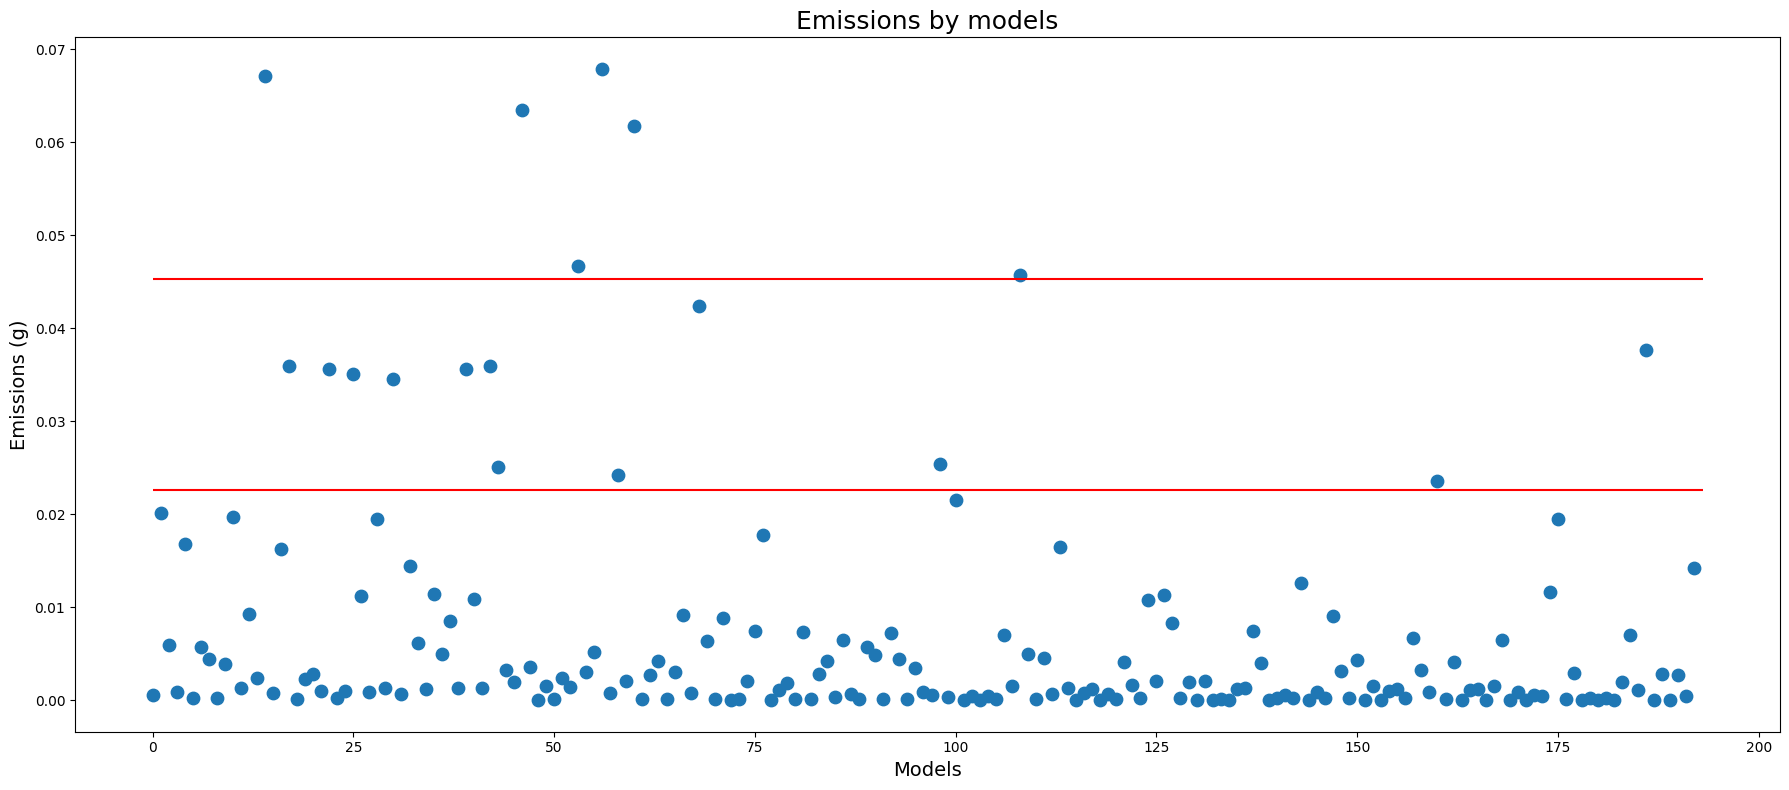
\includegraphics[width=\textwidth]{images/situazione-attuale.png}
    \caption{Emissioni prodotte dai vari modelli}
\end{figure}

\noindent Gli esperimenti passati sono stati condotti su dataset e modelli presenti all'interno di RecBole.\\I dataset utilizzati per l'addestramento dei modelli sono:
\begin{itemize}
    \item \textbf{MovieLens-1M}
    \item \textbf{Amazon\_Book\_60core\_kg} 
    \item \textbf{Mind}
\end{itemize}

\noindent I modelli utilizzati per l'addestramento sono:
\begin{itemize}
    \item \textbf{BPR} \cite{BPR}: General
    \item \textbf{CDAE} \cite{CDAE}: General
    \item \textbf{CFKG} \cite{CFKG}: Knowledge
    \item \textbf{CKE} \cite{CKE}: Knowledge
    \item \textbf{DGCF} \cite{DGCF}: Knowledge
    \item \textbf{DMF} \cite{DMF}: General
    \item \textbf{DiffRec} \cite{DiffRec}: General
    \item \textbf{ENMF} \cite{ENMF}: General 
    \item \textbf{FISM} \cite{FISM}: General
    \item \textbf{GCMC} \cite{GCMC}: General
    \item \textbf{ItemKNN} \cite{ItemKNN}: General
    \item \textbf{KGCN} \cite{KGCN}: Knowledge
    \item \textbf{KGIN}: \cite{KGIN} Knowledge
    \item \textbf{KGNNLS} \cite{KGNNLS}: Knowledge
    \item \textbf{KTUP} \cite{KTUP}: Knowledge
    \item \textbf{LDiffRec} \cite{LDiffRec}: General
    \item \textbf{LINE} \cite{LINE}: General
    \item \textbf{LightGCN} \cite{LightGCN}: General
    \item \textbf{MKR} \cite{MKR}: Knowledge
    \item \textbf{MacridVAE} \cite{MacridVAE}: General
    \item \textbf{MultiDAE} \cite{MultiDAE}: General
    \item \textbf{MultiVAE} \cite{MultiVAE}: General
    \item \textbf{NCEPLRec} \cite{NCEPLRec}: General
    \item \textbf{NCL} \cite{NCL}: General
    \item \textbf{NGCF} \cite{NGCF}: General
    \item \textbf{NeuMF} \cite{NeuMF}: General
    \item \textbf{Pop}: General
    \item \textbf{Random}: General
    \item \textbf{RecVAE} \cite{RecVAE}: General
    \item \textbf{RippleNet} \cite{RippleNet}: Knowledge
    \item \textbf{SGL} \cite{SGL}: General
    \item \textbf{SLIMElastic} \cite{SLIMElastic}: General
    \item \textbf{SimpleX} \cite{SimpleX}: General
    \item \textbf{SpectralCF} \cite{SpectralCF}: General
    \item \textbf{EASE} \cite{EASE}: General
    \item \textbf{NAIS} \cite{NAIS}: General
    \item \textbf{ADMMSLIM} \cite{ADMMSLIM}: General
    \item \textbf{ConvNCF} \cite{ConvNCF}: General
    \item \textbf{NNCF} \cite{NNCF}: General
\end{itemize}

\noindent In questo ambito  Spillo et al.\cite{spillo2023towards} mostrano come spesso algoritmi più semplici riescono ad avere delle performance molto simili a modelli più complessi, ma con un impatto ambientale decisamente minore. Lo scopo di questo lavoro è dunque quello di confermare o smentire questi risultati.\\
\begin{figure}[H]
    \centering
    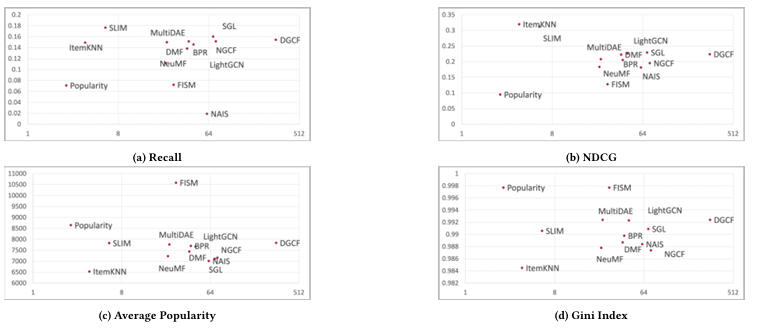
\includegraphics[width=\textwidth]{images/risultati-valutazione.png}
    \caption{Trade-off tra emissioni e performance con dataset Mind}
\end{figure}

\noindent RecBole richiede la definizione di un file di configurazione per poter addestrare i modelli. Questo file di configurazione contiene le seguenti informazioni:\\
\noindent \textbf{Parametri di environment} (servono per configurare l'ambiente di addestramento)
\begin{itemize}
    \item \textbf{gpu\_id}: 0
    \item \textbf{worker}: 0
    \item \textbf{use\_gpu}: True
    \item \textbf{seed}: 2020
    \item \textbf{state}: INFO
    \item \textbf{encoding}: utf-8
    \item \textbf{reproducibility}: True
    \item \textbf{shuffle}: True
\end{itemize}


\noindent \textbf{Parametri di training} (servono per l'addestramento dei modelli)
\begin{itemize}
    \item \textbf{epochs}: 200
    \item \textbf{train\_batch\_size}: 2048
    \item \textbf{learner}: adam
    \item \textbf{learning\_rate}: .001
    \item \textbf{train\_neg\_sample\_args}: 
    \begin{itemize}
        \item \textbf{distribution}: uniform
        \item \textbf{sample\_num}: 1
        \item \textbf{dynamic}: False
        \item \textbf{candidate\_num}: 0
    \end{itemize}
    \item \textbf{eval\_step}: 1
    \item \textbf{stopping\_step}: 10
    \item \textbf{clip\_grad\_norm}: None
    \item \textbf{loss\_decimal\_place}: 4
    \item \textbf{weight\_decay}: .0
    \item \textbf{require\_pow}: False
    \item \textbf{enable\_amp}: False
    \item \textbf{enable\_scaler}: False
\end{itemize}


\noindent \textbf{Parametri di evaluation} (servono per valutare i modelli)


\begin{itemize}
    \item \textbf{eval\_args}:
    \item \begin{itemize}
                \item \textbf{group\_by}: user
                \item \textbf{order}: RO
                \item \textbf{split}: RS : [0.8, 0.1, 0.1]
                \item \textbf{mode}: full
            \end{itemize}
    \item \textbf{repeatable}: False
    \item \textbf{metrics}: ['Recall', 'MRR', 'NDCG', 'Hit', 'MAP', 'Precision', 'GAUC', 'ItemCoverage', 'AveragePopularity', 'GiniIndex', 'ShannonEntropy', 'TailPercentage']
    \item \textbf{topk}: 10
    \item \textbf{valid\_metric}: MRR@10
    \item \textbf{eval\_batch\_size}: 4096
    \item \textbf{metric\_decimal\_place}: 4
\end{itemize}


\noindent \textbf{Iper parametri dei modelli}


\noindent Gli iper parametri dei modelli sono un insieme di parametri che vengono utilizzati per configurare i modelli. La loro configurazione può influenzare il risultato finale. Esistono delle tecniche di HyperTuning che permettono di trovare i migliori iper parametri per un determinato modello e dataset.
In questo caso si è scelto di utilizzare gli iper parametri di default per tutti i modelli.\\Per ognuno dei modelli SOTA scelti (prima elencati) sono stati effettuati run con i seguenti dataset:
\begin{itemize}
    \item \textbf{LFM1b\_artist\_20U50I}
    \item \textbf{LFM1b\_artist\_20U50I\_75strat}
    \item \textbf{LFM1b\_artist\_20U50I\_50strat}
    \item \textbf{LFM1b\_artist\_20U50I\_25strat}
    \item \textbf{ml-10m\_50U10I}
\end{itemize}

\noindent Dopo aver terminato le esecuzioni dei modelli sono stati creati dei grafici per poter confrontare i risultati ottenuti. I grafici sono i due tipi:
\begin{itemize}
    \item \textbf{Grafici a barre:} Questi grafici permettono di confrontare le emissioni dei vari modelli rispetto a ogni dataset.
    \item \textbf{Grafici a dispersione:} Questi dataset permettono di confrontare i trade-off tra emissioni e performance dei vari modelli rispetto a ogni dataset.
\end{itemize}

\noindent Per la valutazione dei modelli sono state utilizzate le seguenti metriche:
\begin{itemize}
    \item \textbf{Recall}: è una metrica che misura la capacità di un modello di raccomandare gli item rilevanti per un utente
    \item \textbf{NDCG}: è una metrica che misura la qualità delle raccomandazioni.
    \item \textbf{Gini Index}: è una metrica che misura l'equità nella distribuzione delle raccomandazioni. Un valore più vicino a zero indica una distribuzione più equa
    \item \textbf{Average Popularity}: è una metrica che misura la popolarità media degli item raccomandati. Un valore alto indica che le raccomandazioni sono concentrate su item popolari.
\end{itemize}



\subsubsection{Addestramento sostenibile}
L'addestramento sostenibile consiste nell'addestrare i modelli di recommendation in modo sostenibile, ovvero cercando di ridurre le emissioni di CO2 prodotte durante l'addestramento senza compromettere le performance dei modelli in modo significativo.
Si è dunque deciso di modificare il criterio di early stopping dei modelli inserendo come variabile anche le emissioni.
Il classico criterio di early stopping prevede di fermare l'addestramento del modello quando lo score ottenuto con il validation set non migliora per un certo numero di epoche consecutive.


\begin{figure}[H]
    \centering
     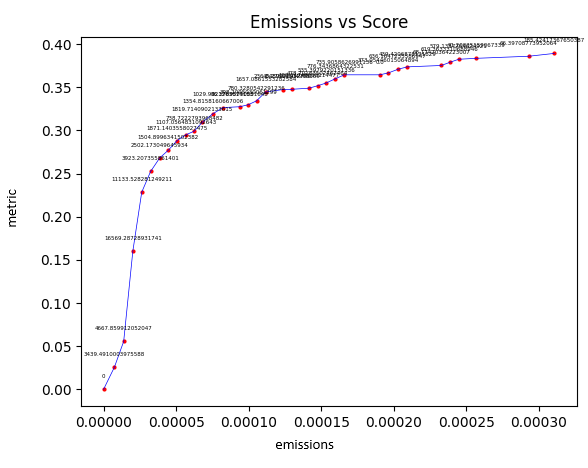
\includegraphics[width=\textwidth]{images/curve_emissions_score.png}
    \caption{Andamento dello score in funzione delle emissioni}
\end{figure}

\noindent Questa curva mostra mostra il comportamento dello score in funzione delle emissioni. In particolare si tiene traccia solo delle epoche in cui lo score è migliorato rispetto al risultato migliore.
Si può notare come la curva presenti una forte crescita iniziale, per poi stabilizzarsi e avere un andamento quasi lineare.
Questo andamento lineare indica dunque un miglioramento molto piccolo dello score rispetto all'aumento delle emissioni.

\noindent Il criterio di early stopping con emissioni si pone dunque come obiettivo quello di fermare l'addestramento del modello quando il miglioramento dello score rispetto alle emissioni è troppo piccolo.
L'idea alla base sarebbe quello di fermare l'addestramento studiando la derivata della curva. Siccome i valori sono discreti, si è deciso di approssimare la derivata con la differenza tra due punti consecutivi \footnote{Metodo delle differenze divise di ordine 1}{} mediante la seguente formula:
\begin{equation}
    \frac{f(x_{i+1}) - f(x_i)}{x_{i+1} - x_i}
\end{equation}

\noindent Quando la differenza tra due rapporti consecutivi è minore di una certa soglia, per un certo numero di volte consecutive, si ferma l'addestramento del modello.\\
\paragraph{Parte esplorativa}
In questa parte si sono eseguti diversi esperimenti usando dataset diversi e parametri diversi per cercare di capire come il criterio di early stopping con emissioni influenzi le performance dei modelli in base ai parametri e alle dimensioni del dataset.\\
\begin{itemize}
    \item \textbf{Primo esperimento}: è stato eseguito con il dataset MovieLens-1m. La soglia è stata impostata a 50 e il numero di epoche consecutive a 5.
    \item \textbf{Secondo esperimento}: è stato eseguito con il dataset LFM-1b\_artist\_20U50I\_25strat. La soglia è stata impostata a 30 e il numero di epoche consecutive a 7, dunque un criterio più stringente (una differenza tra i rapporti consecutivi minore da verificare per più miglioramenti consecutivi).
    \item \textbf{Terzo esperimento}: è stato eseguito sul dataset amazon\_books\_60core\_kg e i parametri utilizzati sono stati 40 come soglia e 6 come numero di epoche consecutive, dunque una via di mezzo tra i due esperimenti precedenti.
\end{itemize}

Per ogni esperimento sono stati realizzati i seguenti grafici:
\begin{itemize}
    \item \textbf{Grafico delle emissioni}: confronta le emissioni prodotte dai vari modelli durante l'addestramento.
    \item \textbf{Grafico del trade-off}: mette in relazione il trade-off tra emissioni e performance dei modelli addestrati con il criterio di early stopping con emissioni e il trade-off dei modelli addestrati con il criterio di early stopping classico.
    \item \textbf{Grafico del decrementi performance}: mostra il decremento delle performance dei modelli addestrati con il criterio di early stopping con emissioni rispetto al criterio di early stopping classico.
\end{itemize}

Anche in questo caso sono state utilizzate le seguenti metriche per valutare i modelli:
\begin{itemize}
    \item \textbf{Recall}
    \item \textbf{NDCG}
    \item \textbf{Gini Index}
    \item \textbf{Average Popularity}
\end{itemize}

\paragraph{Confronto tra i criteri di early stopping con emissioni}
In questa parte parte si è cercato di capire come i parametri del criterio di early stopping con emissioni influenzino le performance dei modelli.\\
Per fare ciò si è deciso di eseguire un esperimento con il dataset MovieLens-1m e di variare i parametri del criterio di early stopping con emissioni.\\
Gli esperimenti eseguti sono stati i seguenti:
\begin{itemize}
    \item \textbf{Primo esperimento}: è stato eseguito con la soglia impostata a 40 e il numero di epoche consecutive a 5.
    \item \textbf{Secondo esperimento}: è stato eseguito con la soglia impostata a 30 e il numero di epoche consecutive a 5.
    \item \textbf{Terzo esperimento}: è stato eseguito con la soglia impostata a 40 e il numero di epoche consecutive a 6.
    \item \textbf{Quarto esperimento}: è stato eseguito con la soglia impostata a 30 e il numero di epoche consecutive a 6.
    \item \textbf{Quinto esperimento}: è stato eseguito con la soglia impostata a 40 e il numero di epoche consecutive a 7.
    \item \textbf{Sesto esperimento}: è stato eseguito con la soglia impostata a 30 e il numero di epoche consecutive a 7.
\end{itemize}

\noindent Sono stati prodotti gli stessi grafici degli esperimenti precedenti per poter confrontare i risultati ottenuti. Sono state utilizzate le stesse metriche degli esperimenti precedenti per valutare i modelli.

\paragraph{Studio della sensibilità dei parametri}
\noindent Per poter confrontare i risultati ottenuti e come i parametri influenzino le performance dei modelli sono stati realizzati dei grafici che mettono in relazione i trade-off tra emissioni e performance dei modelli addestrati con i diversi parametri del criterio di early stopping con emissioni, in modo da osservare la sensibilità dei parametri.
